\section{Evaluation}
\label{eval}
We have discussed a potential loophole in android's custom provider data flow, in this paper. In order to demonstrate this problem we built a proof-of-concept(PoC). All our experiments were ran on a LG Nexus 5 device with Android Marshmallow 6.0 installed on it. In our PoC, we have an app(COMMAND) that has an exported content provider. We created another app(Parser) that is capable of accessing the content provider. We use two different application package sets and observe the results. The first set contains the COMMAND app without any permission specification and Parser app without any permission request. The second set contains the COMMAND app with permission specification and association with the provider that was created. It also includes the Parser app with the request for the permission created by COMMAND.

\begin{figure}
\centering
\begin{minipage}{.45\columnwidth}
	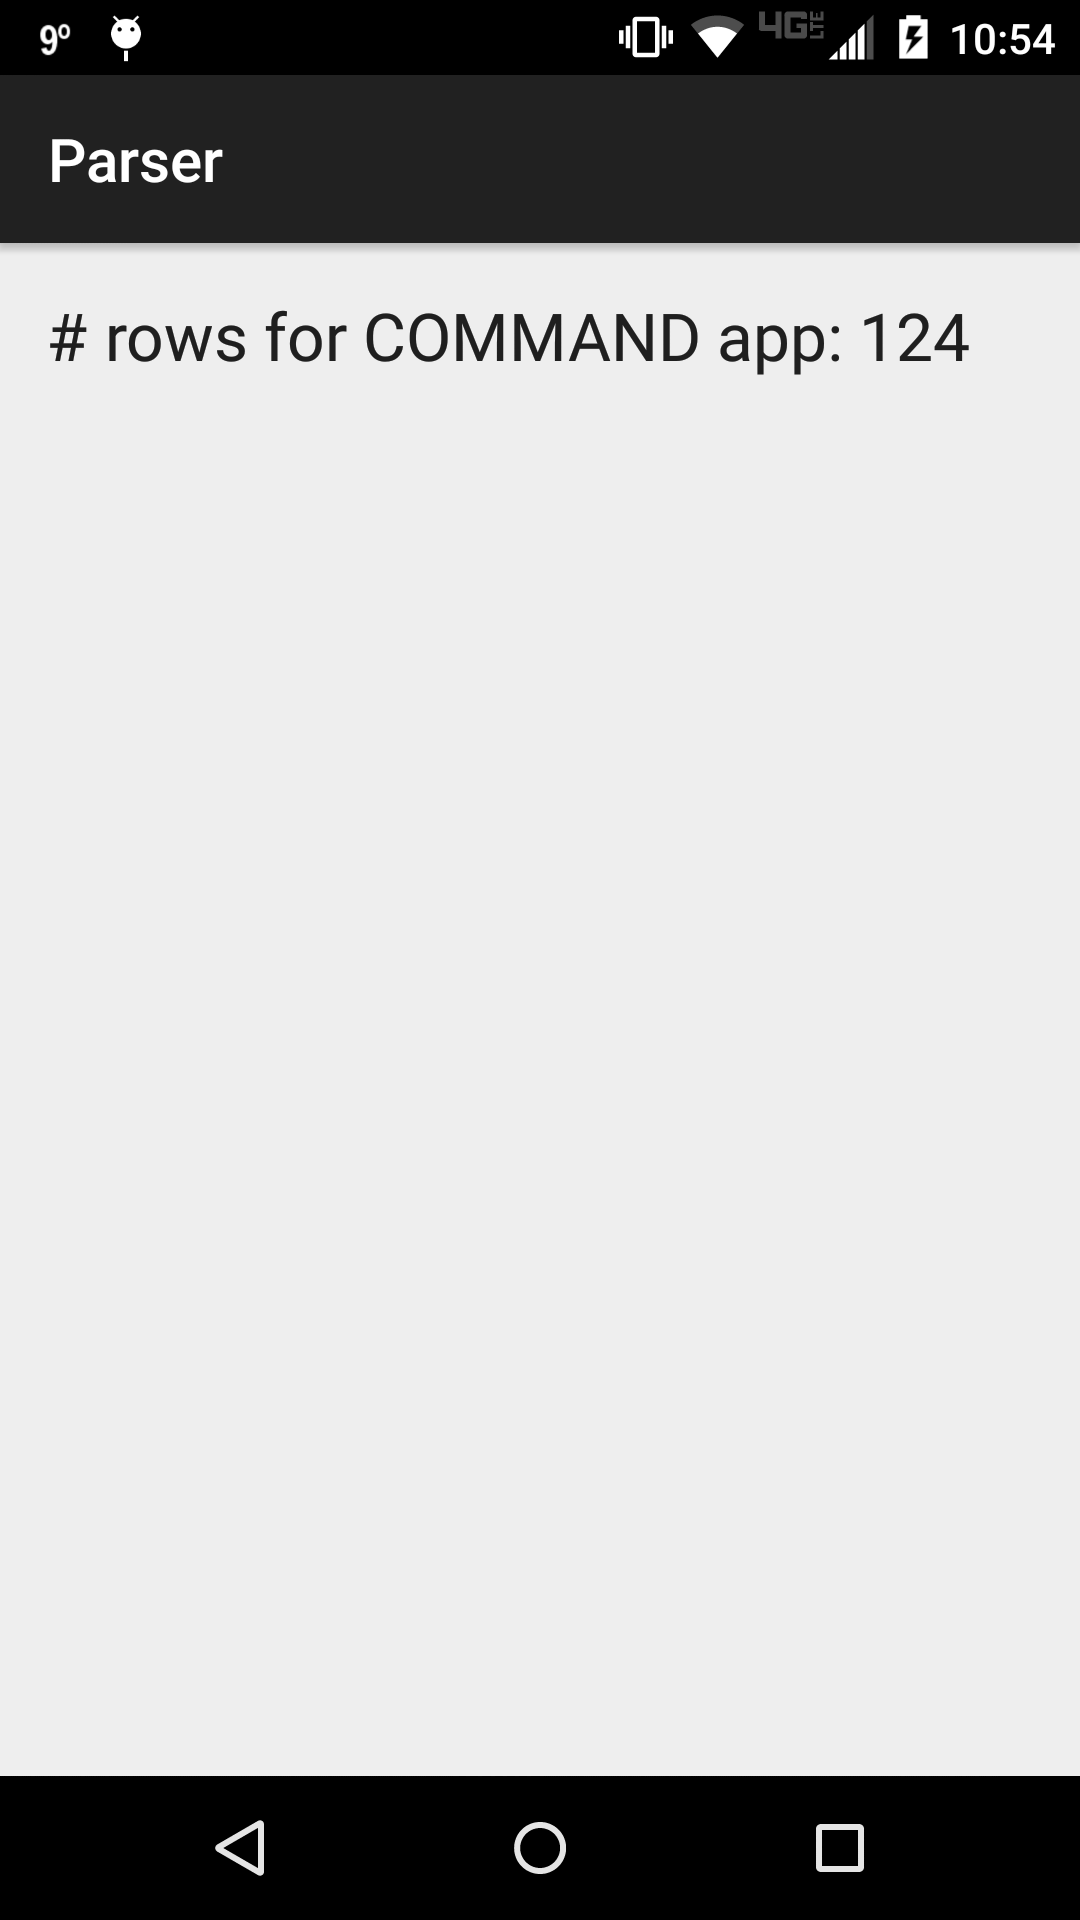
\includegraphics[width=\columnwidth,scale=0.5]{images/bothHavePerm}
	\caption{Android content provider accessed with permission}
	\label{fig:bothHavePerm}
\end{minipage}
\hspace{.05\linewidth}
\begin{minipage}{.45\columnwidth}
	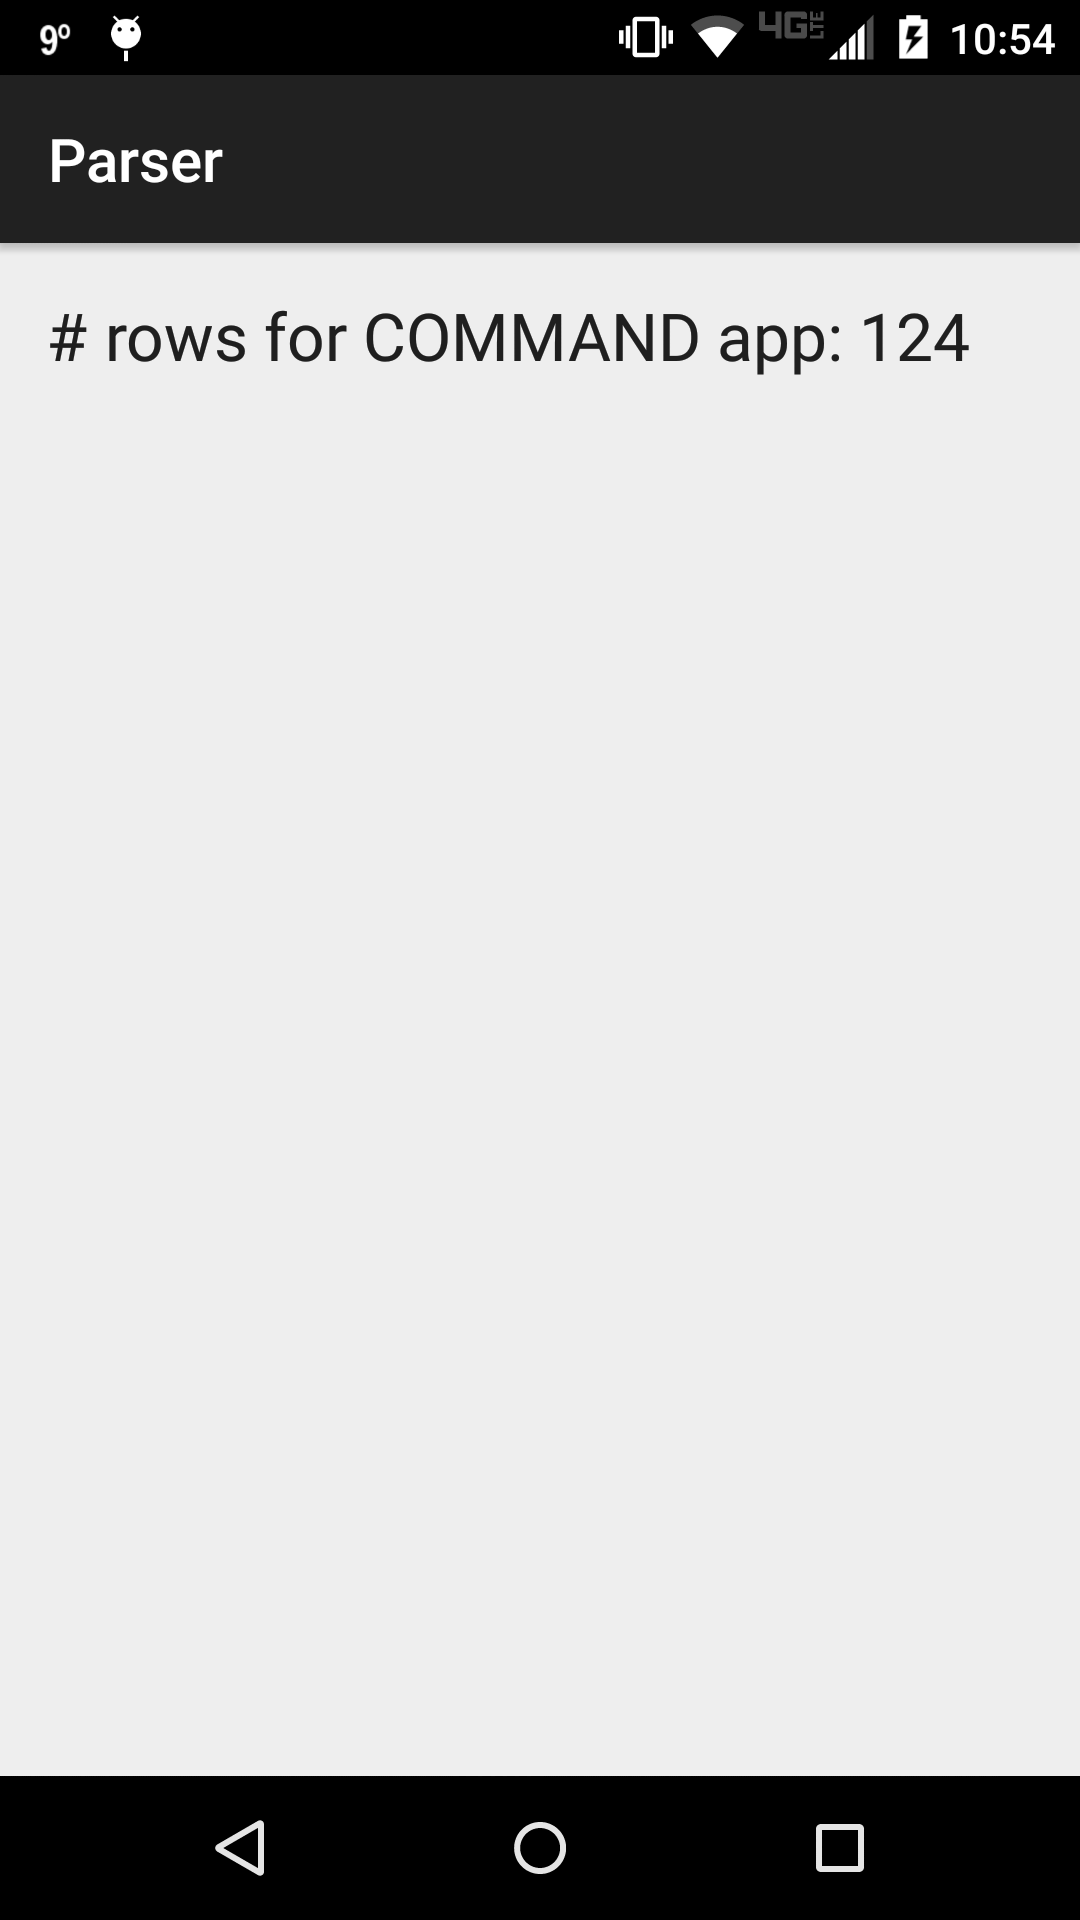
\includegraphics[width=\columnwidth,scale=0.5]{images/neitherHavePerm}
	\caption{Android content provider accessed without permission}
	\label{fig:neitherHavePerm}
\end{minipage}
\end{figure}

\begin{itemize}
	\item Case 1: COMMAND has associated permission, Parser has requested said permission. We see in Figure~\ref{fig:bothHavePerm} that, in this case there are no errors and we are able to make a sample query to the content provider.
	\item Case 2: COMMAND has no associated permission, Parser has not requested said permission. We see in Figure~\ref{fig:neitherHavePerm} that, in this case there are no errors and we are again able to make a sample query to the content provider. We propose that there should a check in such a case to ensure that data access is to be allowed or denied. At present this does not happen and app developers resort to individual techniques to protect their data.
	\item Case 3: COMMAND has associated permission, Parser has not requested said permission. We see in Figure~\ref{fig:didNotRequestPermission} that, causes a permission denial error which is what we expected.
	\item Case 4: COMMAND has no associated permission, Parser has requested an unknown permission. There is no error in this case on the phone. We can ignore this error because this does not cause any leakage from the data provider perspective.
\end{itemize}

\begin{figure}[tb]
\centering
	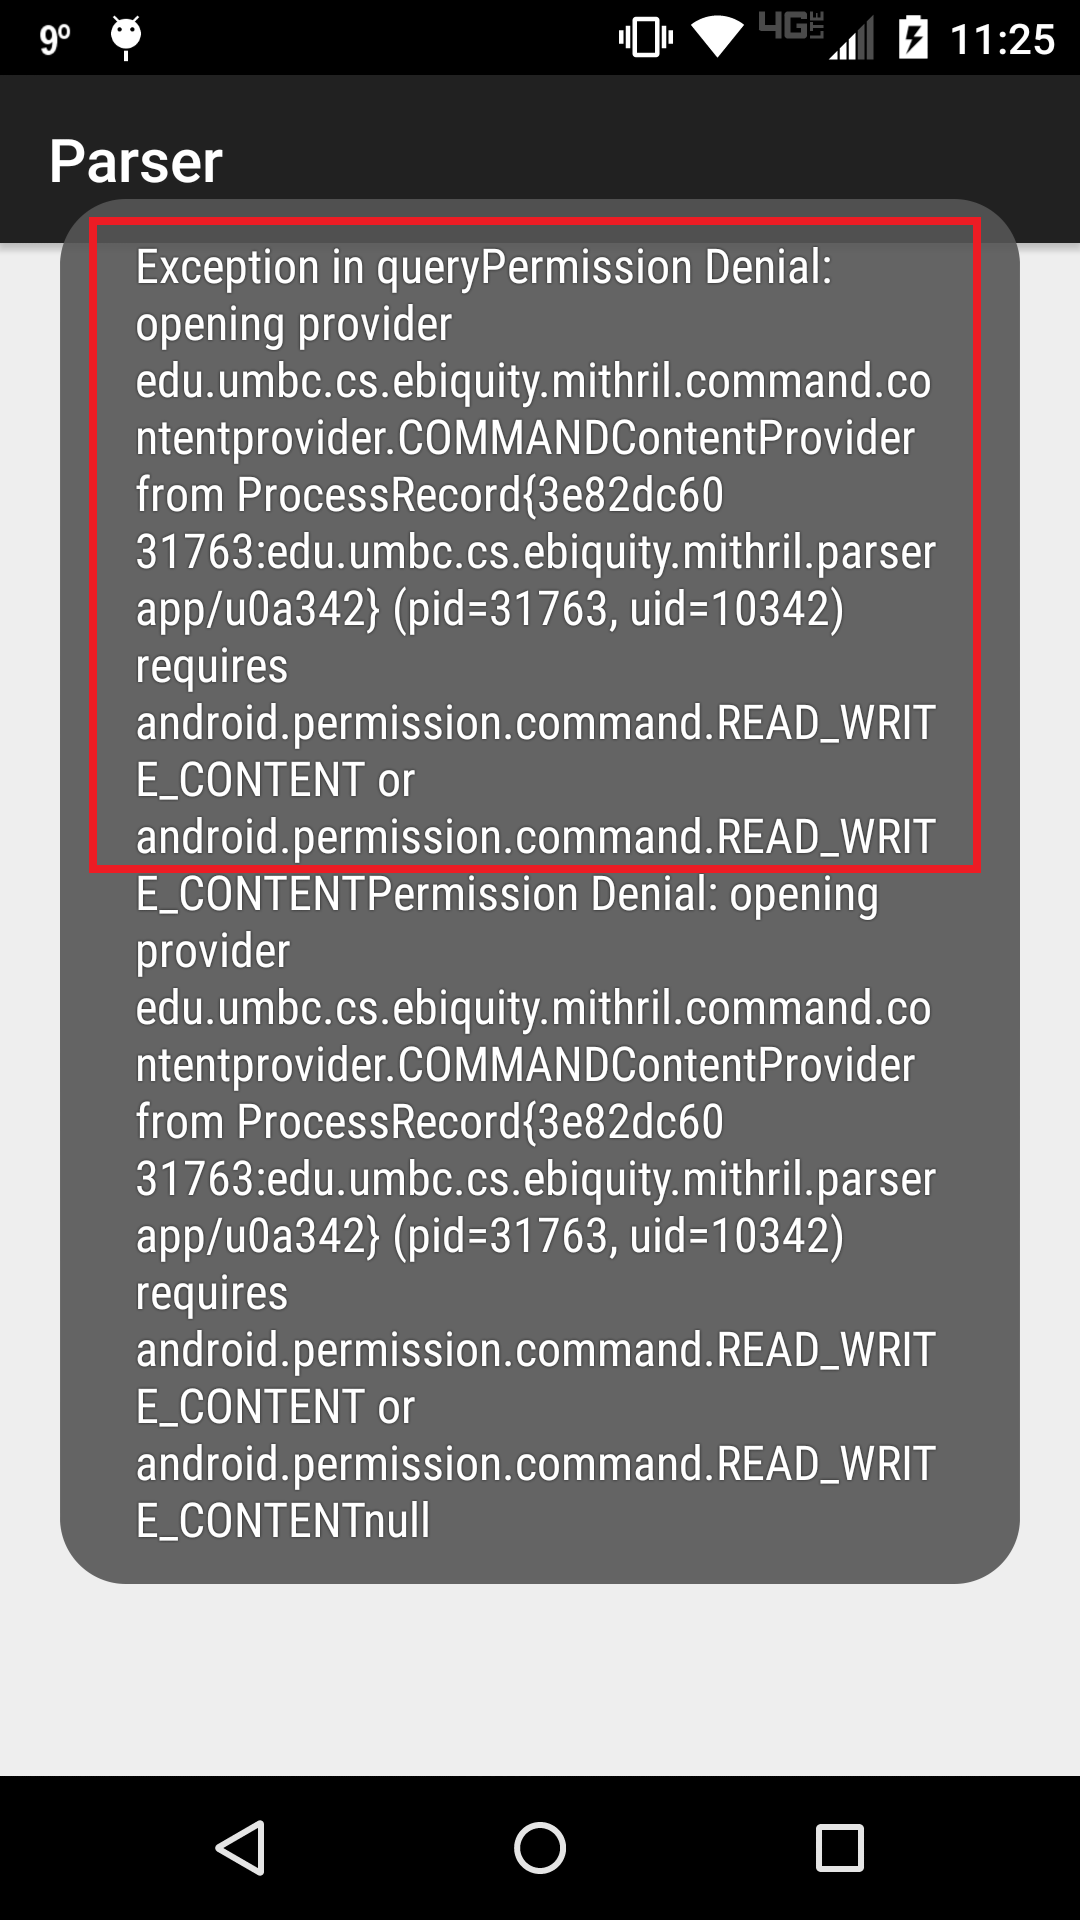
\includegraphics[scale=0.18]{images/didNotRequestPermission}
	\caption{Android content provider permission denial}
	\label{fig:didNotRequestPermission}
\end{figure}

The PoC proves that there is no difference from user perspective between an app which has a content provider with proper protection using appropriate permission and an app which does not have such access control implemented. Therefore, user data can potentially leak without user knowledge.

We also ran our analysis on a set of 1500 randomly selected applications with a mix of popular applications like Facebook, GMail, Instagram as well as less popular and unknown apps like Expense Manager, Call App etc. Our system found 150 applications with provider set as exported and no associated permission for the provider. Therefore about 10\% of apps have this potential loophole but we wanted to find out if we could change an app to leak it's data. This led to our second set of experiments in trying to determine if these had incorporated additional protection apart from the standard android permission mechanisms. For these experiments we used the Facebook app and the Google Fit app. We removed all permissions associated with the providers on both the apps. We also set all the providers' exported setting to true. When these modified apps were installed on our test phone the Google fit app immediately crashed. We used logcat, the Android logging system that provides a mechanism for collecting and viewing system debug output, to observe what was happening on the phone and the cause of the errors. For Google Fit we found that there is an additional check on the key signature that the app is carrying out and it simply crashes because the signature is detected as unknown. You can see the error in Figure~\ref{fig:GoogleProtections}.

\begin{figure}[tb]
\centering
	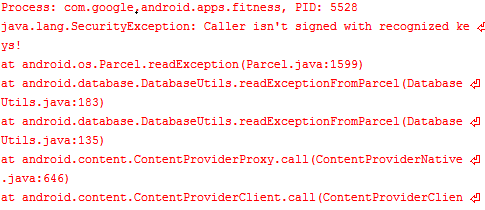
\includegraphics[width=\columnwidth]{images/GoogleProtections}
	\caption{Google Fit app checks for certificate signatures}
	\label{fig:GoogleProtections}
\end{figure}

\begin{figure}[tb]
\centering
	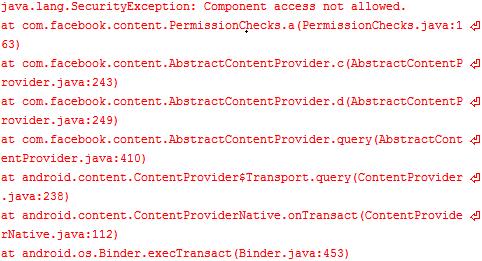
\includegraphics[width=\columnwidth]{images/FBProtections}
	\caption{Facebook checks controls access to it's component}
	\label{fig:FBProtections}
\end{figure}

On the other hand the Facebook app does not ever crash and works like a normal Facebook app. However, when we try to access the app's content provider it blocks our attempt and we can see in Figure~\ref{fig:FBProtections} that it controls access to it's own component. Therefore, app developers are clearly detecting such issues on their apps but not always. We found at least one app that we were able to get access to from our randomly selected apps collection. This app is an Expense Management app and when we tried to access it's content provider we got no checkpoints or errors. Although, as seen in Figure~\ref{fig:nochecks}, our query failed but that was because the app wasn't writing it's data to it's database.

\begin{figure}[tb]
\centering
	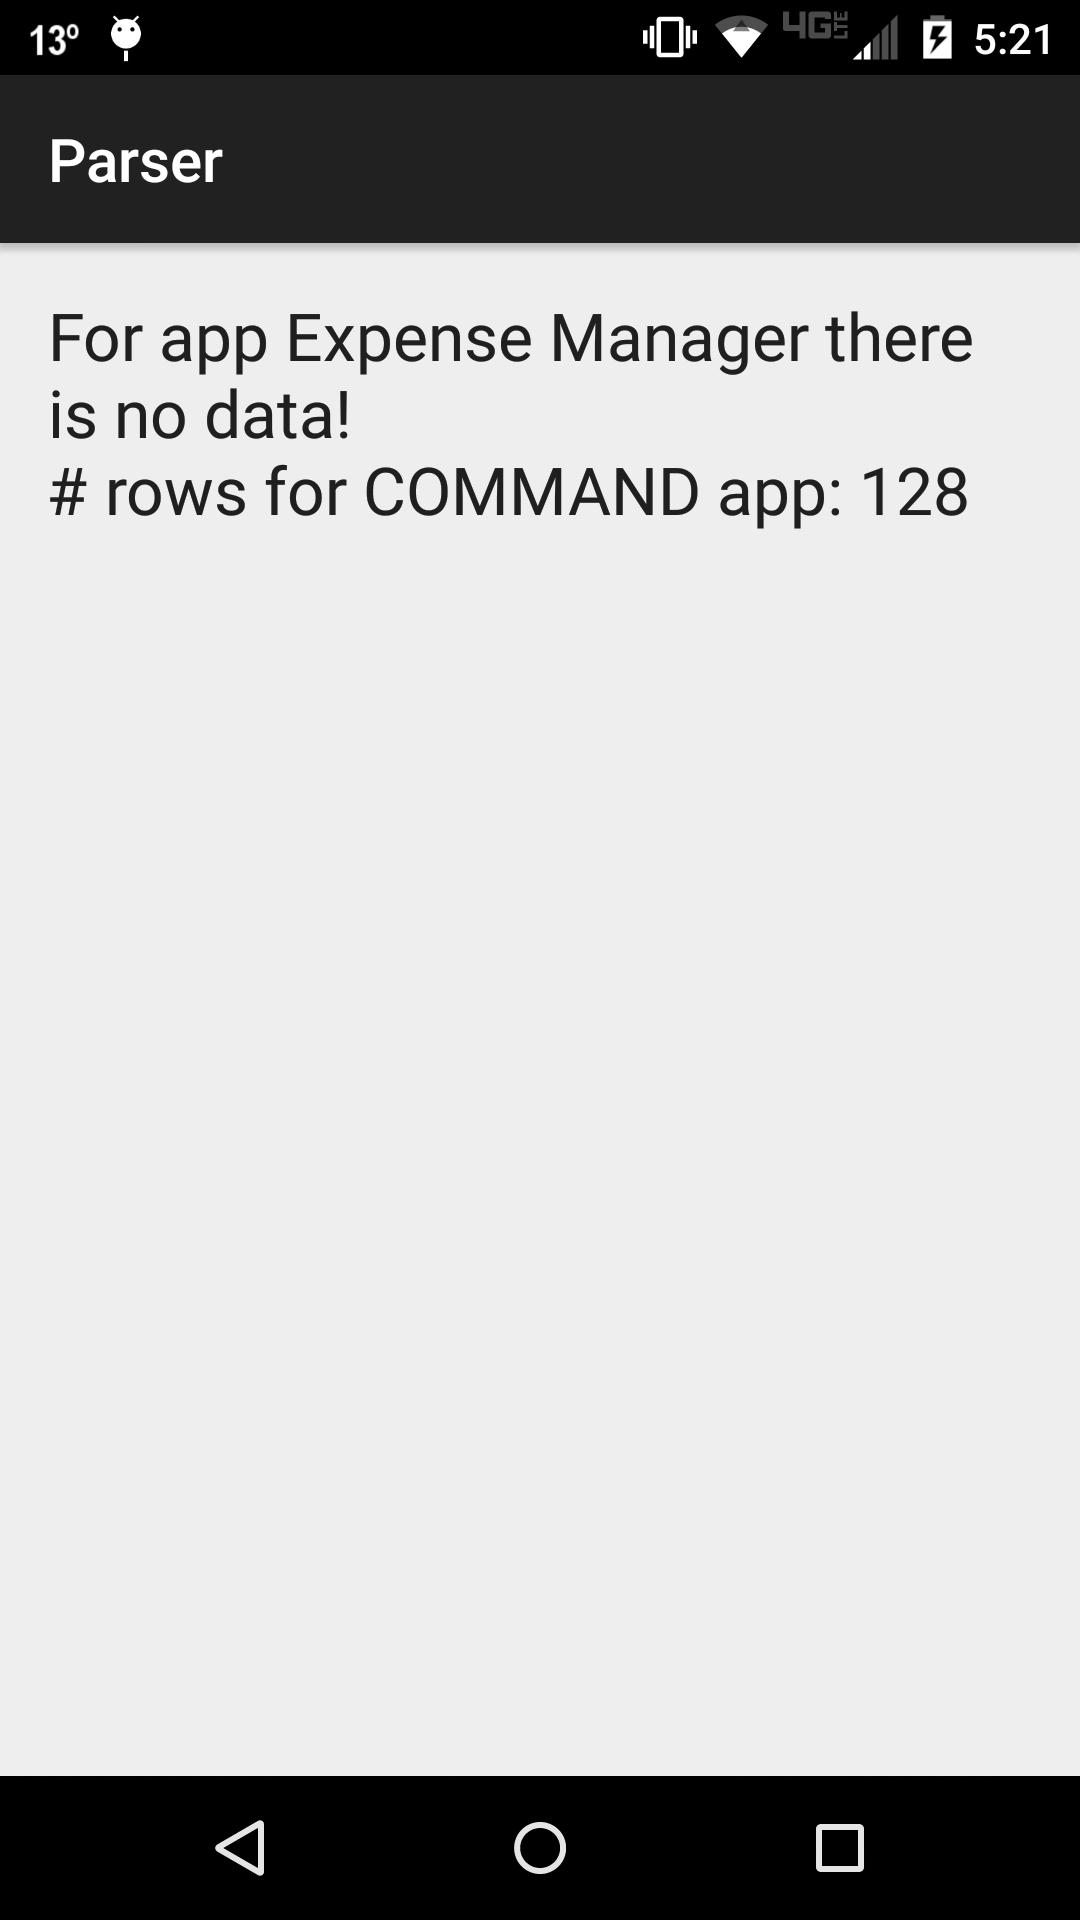
\includegraphics[scale=0.18]{images/nochecks}
	\caption{No check points were found on a less popular app}
	\label{fig:nochecks}
\end{figure}

We are currently processing more apps to find out if they include such checks as encoded by popular apps from Google or Facebook. This processing takes a long time as because we have to manually find the databases on the phone using a rooted phone and a SQLite explorer app. Thereafter, we have to make guesses for patterns that apps might have used in their content provider code. There are commonly used patterns like `\#' that can be used to get access to the data and we are trying to use them to find out apps which have such a vulnerability.